\documentclass[xcolor=pdftex,dvipsnames,table]{beamer}
 \usetheme{Warsaw}
 \usecolortheme[RGB={0,78,0}]{structure}
% \usefonttheme{structurebold}
 %\useoutertheme{smoothbars}
 \useinnertheme{rounded}
\usepackage{amsfonts}
\usepackage{amsmath}
\usepackage{amssymb}
\usepackage{amsthm}
\usepackage{setspace}
\usepackage{graphicx}
\usepackage{url}
\usepackage{mathtools}
\usepackage[]{algorithmicx}
\usepackage{algorithm}
\usepackage{algpseudocode}
\usetheme{Warsaw}
%\usecolortheme{beaver}

\setbeamertemplate{theorems}[numbered]

\theoremstyle{plain}
\newtheorem{thm}{Theorem}
\newtheorem{cor}[thm]{Corollary}
\newtheorem{lem}[thm]{Lemma}
\newtheorem{prop}[thm]{Proposition}

\theoremstyle{definition}
\newtheorem{defn}{Definition}
\newtheorem{defns}{``Definition"}

\def\CC{\mathbb{C}}
\def\RR{\mathbb{R}}
\def\ZZ{\mathbb{Z}}
\def\NN{\mathbb{N}}
\def\QQ{\mathbb{Q}}
\def\FF{\mathbb{F}}
\def\KK{\mathbb{K}}

\newcommand{\set}[1]{\lbrace #1 \rbrace}
\newcommand{\paren}[1]{\left( #1 \right)}
\newcommand{\brac}[1]{\left[ #1 \right]}
\newcommand{\angl}[1]{\langle #1 \rangle}
\newcommand{\abs}[1]{\left| #1 \right|}

\begin{document}

\title[Elliptic Curves] % (optional, only for long titles)
{Elliptic Curves}
%\subtitle{Text Here}
\author[McCarthy] % (optional, for multiple authors)
{Matthew McCarthy}
\institute[CNU] % (optional)
{
  Christopher Newport University
}
\date[11/14/15] % (optional)
{CNU Math Contest\\ November 2015}

%\subject{Mathematics}

\frame{\titlepage}

\begin{frame}
	\frametitle{Algebraic Structures}

	\begin{defns}[Set]
		A \textit{set} is a gathering of distinct numbers.
	\end{defns}
	\begin{defns}[Group]
		A \textit{group} is a set of numbers in which we can add and subtract any two numbers while remaining inside the set.
	\end{defns}
	\begin{defns}[Field]
		A \textit{field} is a set of numbers in which we can add, subtract, multiply, and divide any two numbers (excluding division by zero) while remaining inside the set.
	\end{defns}
\end{frame}

\begin{frame}
	\frametitle{Working Definition of an Elliptic Curve}

	\begin{defns}[Elliptic Curve (from \cite{AEC})]
		An \textit{elliptic curve} over a field $\FF$ is a nonsingular cubic equation of the form
		\begin{equation}\label{WEQN}
		y^2+a_1xy+a_3y=x^3+a_2x^2+a_4x+a_6
		\end{equation}
		where $a_1,a_2,a_3,a_4,a_6\in\FF$.
	\end{defns}
	\begin{defn}
		An equation of the form of Equation \autoref{WEQN} is called a \textit{Weierstrass equation}.
	\end{defn}
\end{frame}

\begin{frame}
	\frametitle{Kinds of Elliptic Curves over $\RR$}
	\begin{columns}
	\column{0.3\textwidth}
	\begin{figure}
		\centering
		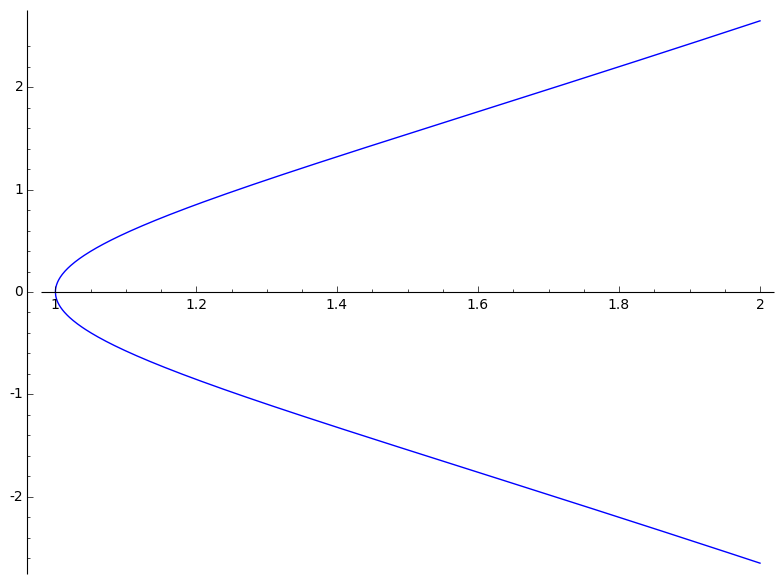
\includegraphics[scale=0.1]{c1.png}
		\caption{$y^2=x^3-1$}
	\end{figure}
	\begin{figure}
		\centering
		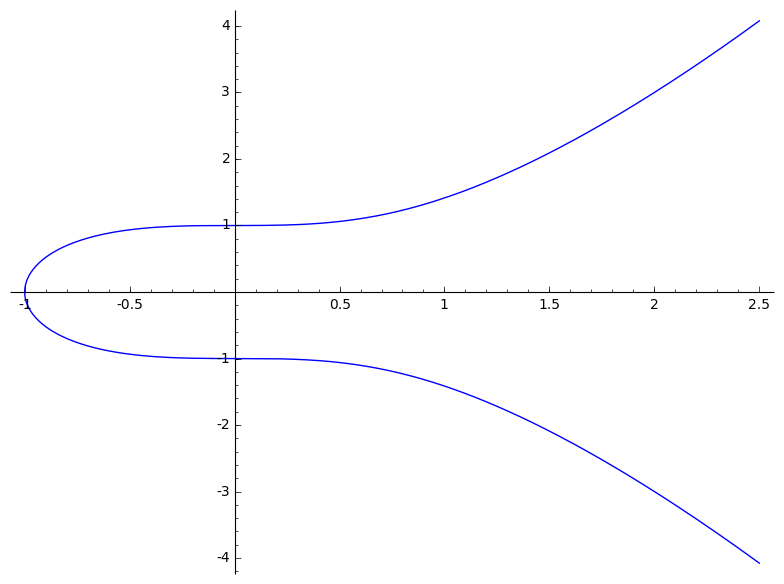
\includegraphics[scale=0.1]{c2.png}
		\caption{$y^2=x^3+1$}
	\end{figure}
	\column{0.3\textwidth}
	\begin{figure}
		\centering
		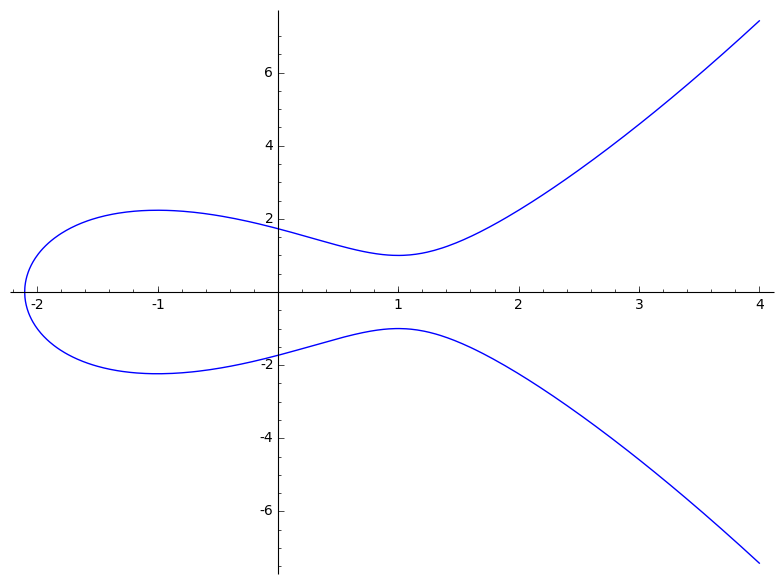
\includegraphics[scale=0.1]{c3.png}
		\caption{$y^2=x^3-3x+3$}
	\end{figure}
	\begin{figure}
		\centering
		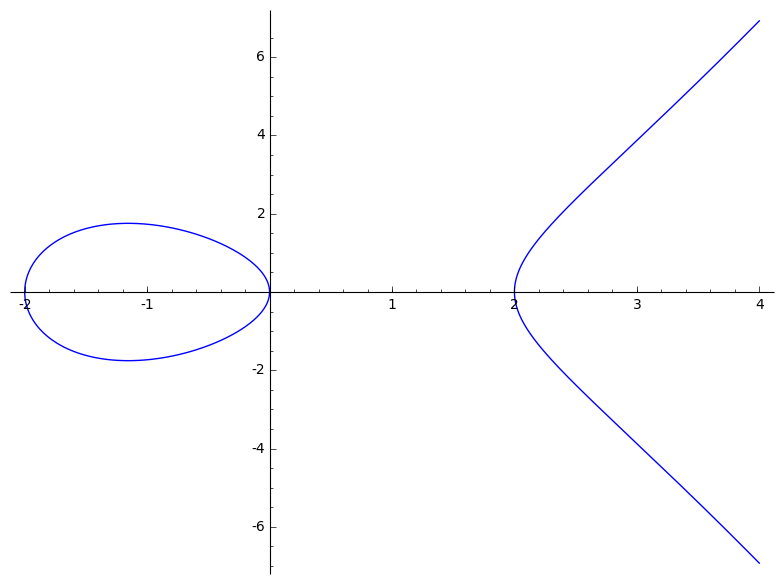
\includegraphics[scale=0.1]{c4.png}
		\caption{$y^2=x^3-4x$}
	\end{figure}
	\column{0.3\textwidth}
	\begin{figure}
		\centering
		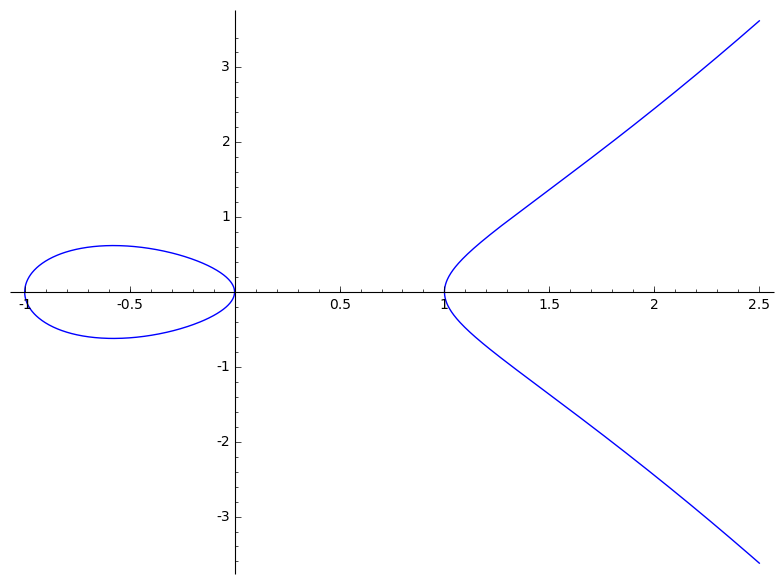
\includegraphics[scale=0.1]{c5.png}
		\caption{$y^2=x^3-x$}
	\end{figure}
	\end{columns}
\end{frame}

\begin{frame}
	\frametitle{Chord and Tangent Rule}

	An elliptic curve over a field forms a group under the chord and tangent rule \cite{Galbraith}.
	\begin{columns}
	\column{0.2\textwidth}
	\begin{figure}
		\centering
		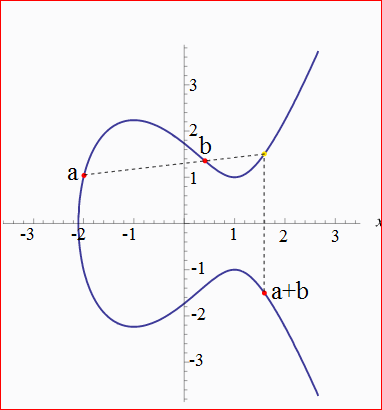
\includegraphics[scale=.2]{p_plus_q.png}
		\caption{$a+b$}
	\end{figure}

	\column{0.2\textwidth}
	\begin{figure}
		\centering
		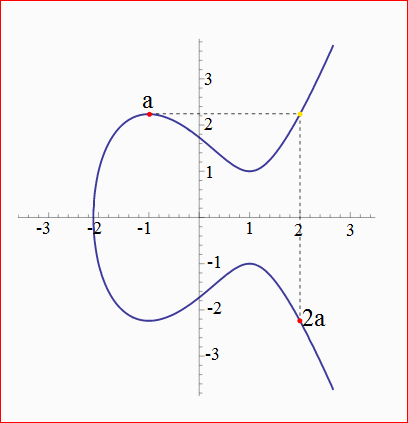
\includegraphics[scale=.2]{p_plus_p.png}
		\caption{$2a$}
	\end{figure}
	\column{0.2\textwidth}
	\begin{figure}
		\centering
		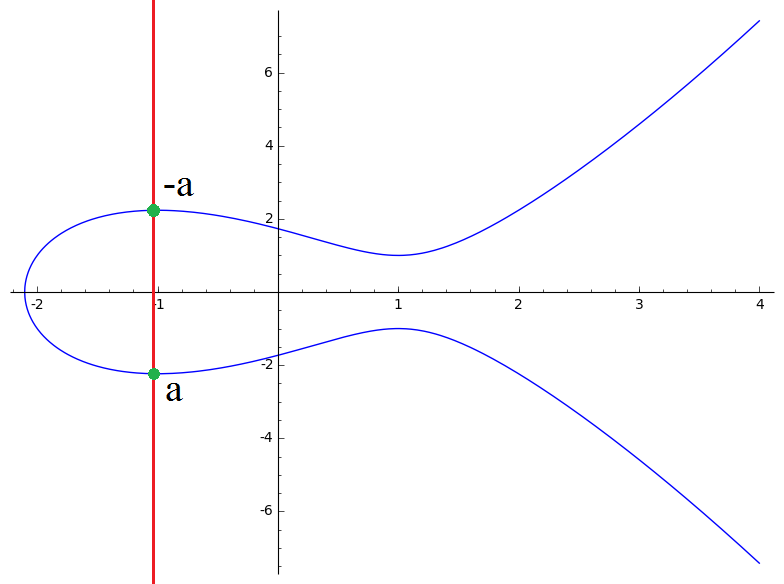
\includegraphics[scale=.16]{p_minus_p.png}
		\caption{$a-a$}
	\end{figure}
	\end{columns}
\end{frame}

\begin{frame}
	\begin{center}
		\begin{Large}
		Where will the chord between $a$ and $-a$ intersect the curve again?\\[2em]
		\pause
		Where do parallel lines meet?\\[2em]
		\end{Large}
		\pause
		\begin{LARGE}
		At infinity!
		\end{LARGE}
	\end{center}
\end{frame}

\begin{frame}
	\frametitle{Fermat's Last Theorem}

	\begin{thm}
	For $n\geq 3$, the equation
	\[
		x^n+y^n = z^n
	\]
	has no solutions when $x$,$y$, and $z$ are natural numbers.
	\end{thm}

	\begin{itemize}
	\item This theorem was conjectured by Pierre de Fermat in 1637
	\item Proved by Andrew Wiles in 1994 using elliptic curves
	\end{itemize}
\end{frame}

\begin{frame}
	\frametitle{Cryptography}

	\begin{itemize}
	\item We call the set of remainders when dividing by a prime, $\ZZ_p$.
	\item The logarithm of a number, $\log y$ is a solution to the equation $e^x=y$.
	\item The discrete logarithm of a point on an elliptic curve is a solution to the equation $kP=Q$.
	\item On elliptic curves over $\ZZ_p$, finding the discrete log of a point is hard.
	\end{itemize}

	This means we can use it for cryptography!
\end{frame}

\begin{frame}
	\frametitle{Elgamal}

	\begin{enumerate}
		\item $A$ and $B$ agree on a point $Q$ on an elliptic curve $E$.
		\item $A$ and $B$ choose integers $a$ and $b$ respectively and publish $aQ$ and $bQ$.
		\item $A$ wants to send a message to $B$.
		\begin{itemize}
			\item $A$ embeds message $m$ into a point on $E$, called $P_m$.
			\item $A$ then sends $P_m+a(bQ)$ to $B$.
		\end{itemize}
		\item $B$ wants to retrieve the message $A$ sent him.
		\begin{itemize}
			\item $B$ computes,
			\[
				(P_m+a(bQ))-b(aQ)=P_m+abQ-abQ=P_m.
			\]
			\item $B$ then reverses the embedding to get back $m$.
		\end{itemize}
	\end{enumerate}
\end{frame}

\begin{frame}[allowframebreaks]
\frametitle{References}
\begin{thebibliography}{10}
	\bibitem{Galbraith}
		Steven D. Galbraith
		\newblock Mathematics of Public Key Cryptography
	\bibitem{ECDSA}
		Richard Schroeppel and Cheryl Beaver
		\newblock Algorithms for Improved Performance in Cryptographic Protocols
		\newblock Sandia National Laboratories. In: SAND REPORT (2003-4283)a
	\bibitem{AEC}
		Joseph H. Silverman
		\newblock The Arithmetic of Elliptic Curves
		\newblock Graduate Texts in Mathematics
	\bibitem{ET}
		Avner {Ash} and Robert {Gross}
		\newblock Elliptic Tales
\end{thebibliography}
\end{frame}

\begin{frame}
\begin{Large}
\begin{center}
Thank you!
\end{center}
\end{Large}
\end{frame}

\end{document}
